\chapter{Contents}
\setlength{\parskip}{12pt}
\setlength{\parindent}{10mm} 
\onehalfspacing

The goal of this chapter is to illustrate the environments for definition, lemma, theorem, corollary, proof, figure, and table.

\section{Definition, Lemma, Theorem, Corollary, and Proof}
Let $\mathbb{N} = \{1, 2, 3, \ldots \}$ be the set of natural numbers.

\begin{definition}[Prime and Composit]
\label{primes and composits}
A natural number is called a {\em prime number} (or a {\em prime}) if it has exactly two positive divisors, $1$ and the number itself \cite{numbertheory-underwoord}.  Natural numbers greater than $1$ that are not prime are called {\em composite}.
\end{definition}

\begin{lemma}[2 is prime]
\label{2-is-prime} 
2 is a prime number.
\end{lemma}

\begin{proof}
2 and 1 are exactly two positive divisors of 2.
\end{proof}

\begin{theorem}[2 is the only even prim number]
\label{2-is-prime} 
An even natural number greater than 2 is not prime.
\end{theorem}

\begin{proof}
Every even natural number is a composite as there are at least three positive divisors: $1$, $2$, and the number itself.
\end{proof}

From Theorem \ref{2-is-prime}, we have the following corollary.

\begin{corollary}[Most of even natural numbers are not prime]
$2$ is the only even prime number.
\end{corollary}

\section{Table and Figure}
Figure \ref{prime-distribution} illustrates the asymtotic distribution of prime numbers according to the \textsc{Prime Number Theorem (PNT)} which is stated as follows:

\begin{theorem}[\textsc{Prime Number Theorem (PNT)}]
Let $\pi(x)$ denote the prime-counting function that gives the number of primes less than or equal to $x$, for any real number $x$.

\[ \lim_{x \to \infty} \frac{\pi(x)}{\frac{x}{\log{(x)}}} = 1\]
\end{theorem}

In other words, the \textsc{PNT} states that $x / \log{x}$ is a good approximation to $\pi(x)$.

\begin{figure}[h!] \vspace{10pt} \centering
\vspace{7pt}
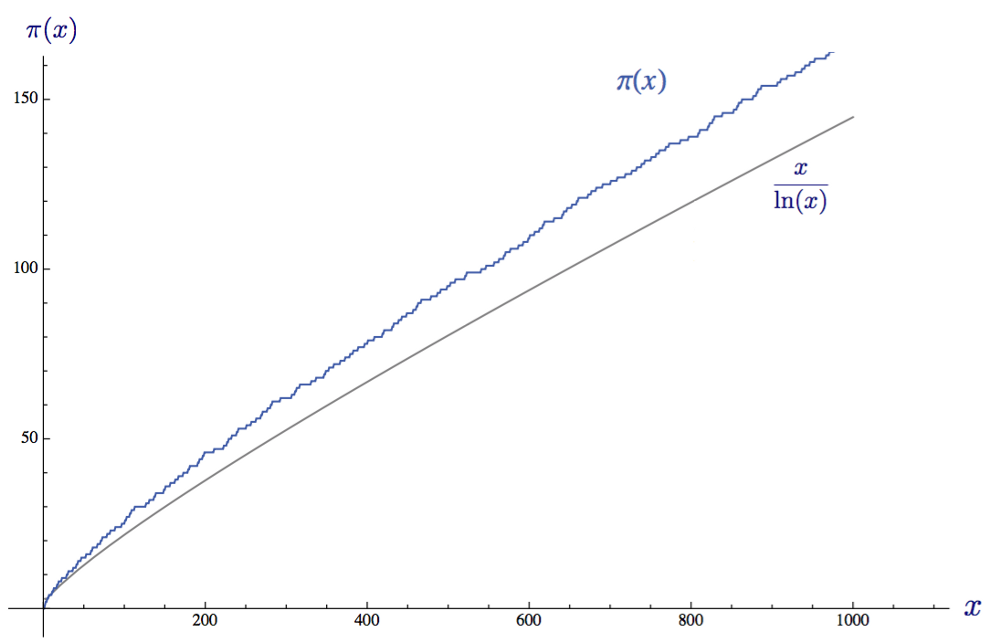
\includegraphics[width=10cm]{figures/prime-number-theorem-absolute.png}
\vspace{7pt}
\caption[Distribution of prime numbers regarding Prime Number Theorem ]{The prime counting function $\pi(x)$ and the estimate from the the \textsc{PNT} plotted up to $x$ = 1000. Source: \url{https://cdn-images-1.medium.com/max/1000/1*AhZ7SxlQWrBGd4HXHs1JWA.png}}
\label{prime-distribution}
\vspace{-5mm}
\end{figure}

The following table shows all prime numbers up to 1000.

\begin{table}[h!]
\vspace{-2mm}
\begin{center}
\caption[All prime numbers up to 1000.]{All prime numbers up to 1000.}
\begin{tabular}{| c | c | c | c | c | c | c | c | c | c |}
\hline
& 2 & 3 & 5 & 7 & 11 & 13 & 17 & 19 & 23 \\
29 & 31 & 37 & 41 & 43 & 47 & 53 & 59 & 61 & 67 \\
71 & 73 & 79 & 83 & 89 & 97 & 101 & 103 & 107 & 109 \\
113 & 127 & 131 & 137 & 139 & 149 & 151 & 157 & 163 & 167 \\
173 & 179 & 181 & 191 & 193 & 197 & 199 & 211 & 223 & 227 \\
229 & 233 & 239 & 241 & 251 & 257 & 263 & 269 & 271 & 277 \\
281 & 283 & 293 & 307 & 311 & 313 & 317 & 331 & 337 & 347 \\
349 & 353 & 359 & 367 & 373 & 379 & 383 & 389 & 397 & 401 \\
409 & 419 & 421 & 431 & 433 & 439 & 443 & 449 & 457 & 461 \\
463 & 467 & 479 & 487 & 491 & 499 & 503 & 509 & 521 & 523 \\
541 & 547 & 557 & 563 & 569 & 571 & 577 & 587 & 593 & 599 \\
601 & 607 & 613 & 617 & 619 & 631 & 641 & 643 & 647 & 653 \\
659 & 661 & 673 & 677 & 683 & 691 & 701 & 709 & 719 & 727 \\
733 & 739 & 743 & 751 & 757 & 761 & 769 & 773 & 787 & 797 \\
809 & 811 & 821 & 823 & 827 & 829 & 839 & 853 & 857 & 859 \\
863 & 877 & 881 & 883 & 887 & 907 & 911 & 919 & 929 & 937 \\
941 & 947 & 953 & 967 & 971 & 977 & 983 & 991 & 997 & \\
\hline
\end{tabular}
\end{center}
\vspace{-7mm}
\end{table}





